\makeatother
%	\author{Mitesh M. Khapra}
	\title{Module 3}
	\subtitle{The Deep Revival}
		\author{}
		\institute{}
	\date{}
%\institute{Department of Computer Science and Engineering\\ Indian Institute of Technology Madras}
%\titlegraphic{
\includegraphics[height=1cm,width=2cm]{images/iitm_logo.png}}
%\titlegraphicii{\includegraphics[height=1cm,width=2cm]{logo2}}

\begin{frame}
	\myheading{Chapter 3: The Deep Revival}
\end{frame}

\begin{frame}
	\begin{minipage}[t][0.6\textheight][t]{\textwidth}
		\begin{columns}
			\column{0.5\textwidth}
				\begin{overlayarea}{\textwidth}{\textheight}
					\justify
					\only<1>{\myheading{Unsupervised Pre-Training}}
					\only<1>{Hinton and  Salakhutdinov described an effective way of initializing the weights that allows deep autoencoder networks to learn a low-dimensional representation of data. \cite{Salakhutdinov:2012:ELP:2330716.2330717}}
				\end{overlayarea}
			\column{0.5\textwidth}
					\begin{overlayarea}{\textwidth}{\textheight}
						\begin{figure}
							\centering
							\only<1>{\includegraphics[scale=0.7]{"images/Renewed_Interest/2006_1"}
						\end{figure}
					\end{overlayarea}
		\end{columns}
	\end{minipage}
	\begin{minipage}[t][0.4\textheight][t]{\textwidth}
		\begin{columns}
		\column{0.1\textwidth}
		\column{0.9\textwidth}
			\begin{overlayarea}{\textwidth}{\textheight}
			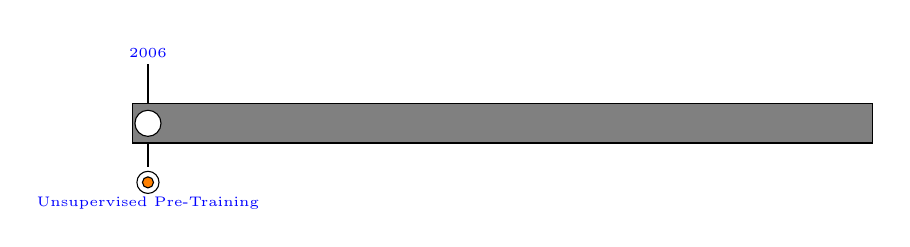
\begin{tikzpicture}[datemarker/.style={circle, draw=black,fill=white},textlabel/.style={anchor=center,text height=1.7ex,text depth=.25ex}] 
			\tikzset{every node/.style={font=\tiny, color=blue}}\draw[fill=gray](-0.2,0) rectangle (9.2,0.5) node[white, below]{}; 
			\onslide<1>{\node at (0.0, 0.25) [datemarker] {};}
			\onslide<1>{\draw [line width=1pt] (0.0, 0.5) to (0.0, 1.0);} 
			\onslide<1>{\draw (0.0, 1.2) node [textlabel] {2006 };}
			\onslide<1>{\draw [fill=orange](0.0, -0.5) circle (2pt){};}
			\onslide<1>{\draw (0.0, -0.5) circle (4pt){};}
			\onslide<1>{\draw [line width=1pt] (0.0, 0) to (0.0, -0.3);}
			\onslide<1>{\draw (0.0,-0.7) node [textlabel] {Unsupervised Pre-Training};}
			\end{tikzpicture}
			\end{overlayarea}
		\end{columns}
	\end{minipage}
\end{frame}
\begin{frame}
\begin{minipage}[t][0.6\textheight][t]{\textwidth}
\begin{columns}
\column{0.5\textwidth}
\begin{overlayarea}{\textwidth}{\textheight}
\justify
\only<1>{\myheading{Unsupervised Pre-Training}}
\only<1>{The idea of unsupervised pre-training actually dates back to 1991-1993 (J. Schmidhuber) when it was used to train a ``Very Deep Learner''}
\only<2>{\myheading{More insights (2007-2009)}}
\only<2>{Further Investigations into the effectiveness of Unsupervised Pre-training}

\only<3>{\myheading{Success in Handwriting Recognition}}
\only<4>{\myheading{Success in Speech Recognition}}
\only<5>{\myheading{ New record on MNIST }}
\only<6>{\myheading{ First Superhuman Visual Pattern Recognition}}
\only<7->{\myheading{Winning more visual recognition challenges}}

\only<3>{Graves et. al. outperformed all entries in an international Arabic recognition competition \cite{NIPS2008_3449}}
\only<4>{Dahl et. al. showed relative error reduction of 16.0\% and 23.2\% over a state of the art system \cite{Dahl:2012:CPD:2335874.2336015}}
\only<5>{Ciresan et. al. set a new record on the MNIST dataset using good old backpropagation on GPUs (GPUs enter the scene)\cite{DBLP:journals/corr/abs-1003-0358}}
\only<6>{D. C. Ciresan et. al. achieved 0.56\% error rate in the IJCNN Traffic Sign Recognition Competition \cite{DBLP:journals/corr/abs-1202-2745}}
\only<7->{\begin{table}
\begin{tabular}{ccc}
\textbf{Network}&\textbf{Error}&\textbf{Layers}\\
\onslide<7->{AlexNet \cite{NIPS2012_4824}}&\onslide<7->{16.0\%}&\onslide<7->{8}\\
\onslide<8->{ZFNet \cite{DBLP:journals/corr/ZeilerF13}}&\onslide<8->{11.2\%}&\onslide<8->{8}\\
\onslide<9->{VGGNet \cite{DBLP:journals/corr/SimonyanZ14a}}&\onslide<9->{7.3\%}&\onslide<9->{19}\\
\onslide<10->{GoogLeNet \cite{DBLP:journals/corr/SzegedyLJSRAEVR14}}&\onslide<10->{6.7\%}&\onslide<10->{22}\\
\onslide<11->{MS ResNet \cite{DBLP:journals/corr/HeZRS15}}&\onslide<11->{3.6\%}&\onslide<11->{152!!}\\
\end{tabular}
\end{table}
}




\end{overlayarea}
\column{0.5\textwidth}
\begin{overlayarea}{\textwidth}{\textheight}
\begin{figure}
\centering
\only<1>{\includegraphics[scale=0.7]{"images/Renewed_Interest/2006_1"}}
\only<2>{\includegraphics[scale=0.23]{"images/Renewed_Interest/2007"}}
\only<3>{\includegraphics[scale=0.15]{"images/Renewed_Interest/2009"}}
\only<4>{\includegraphics[scale=0.5]{"images/Renewed_Interest/2010_1"}}
\only<5>{\includegraphics[scale=0.5]{"images/Renewed_Interest/2010"}}
\only<6>{\includegraphics[scale=0.4]{"images/Renewed_Interest/2011"}}
\only<7->{\includegraphics[scale=0.4]{"images/Renewed_Interest/2012_1"}}


\end{figure}
\end{overlayarea}
\end{columns}
\end{minipage}
\begin{minipage}[t][0.4\textheight][t]{\textwidth}
\begin{columns}
\column{0.1\textwidth}
\begin{overlayarea}{\textwidth}{\textheight}
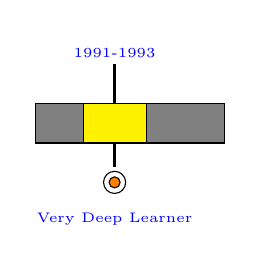
\begin{tikzpicture}[datemarker/.style={circle, draw=black,fill=white},textlabel/.style={anchor=center,text height=1.7ex,text depth=.25ex}]
\tikzset{every node/.style={font=\tiny, color=blue}}\draw[fill=gray](-0.2,0) rectangle (2.2,0.5) node[white, below]{};
%\onslide<1->{\node at (0.0, 0.25) [datemarker] {};}
%\onslide<1->{\draw [line width=1pt] (0.0, 0.5) to (0.0, 1.0);}
%\onslide<1->{\draw (0.0, 1.2) node [textlabel] {1990 };}
%\onslide<1->{\draw [fill=orange](0.0, -0.5) circle (2pt){};}
%\onslide<1->{\draw (0.0, -0.5) circle (4pt){};}
%\onslide<1->{\draw [line width=1pt] (0.0, 0) to (0.0, -0.3);}
%\onslide<1->{\draw (0.0,-0.9) node [textlabel] {};}
\onslide<1->{\draw[fill=yellow] (0.4, 0) rectangle (1.2, 0.5){};}
%\onslide<2->{\node at (0.4, 0.25) [datemarker] {};}
\onslide<1->{\draw [line width=1pt] (0.8, 0.5) to (0.8, 1.0);}
\onslide<1->{\draw (0.8, 1.2) node [textlabel] {1991-1993 };}
\onslide<1->{\draw [fill=orange](0.8, -0.5) circle (2pt){};}
\onslide<1->{\draw (0.8, -0.5) circle (4pt){};}
\onslide<1->{\draw [line width=1pt] (0.8, 0) to (0.8, -0.3);}
\onslide<1->{\draw (0.8,-0.9) node [textlabel] {Very Deep Learner};}
\end{tikzpicture}
\end{overlayarea}


\column{0.9\textwidth}
\begin{overlayarea}{\textwidth}{\textheight}
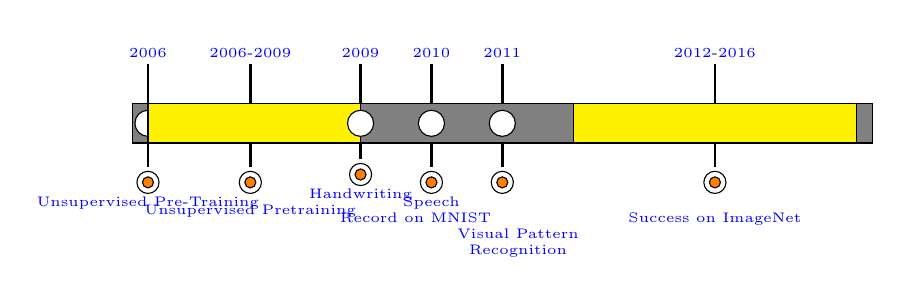
\begin{tikzpicture}[datemarker/.style={circle, draw=black,fill=white},textlabel/.style={anchor=center,text height=1.7ex,text depth=.25ex}] 
\tikzset{every node/.style={font=\tiny, color=blue}}\draw[fill=gray](-0.2,0) rectangle (9.2,0.5) node[white, below]{}; 
\onslide<1>{\node at (0.0, 0.25) [datemarker] {};}
\onslide<1>{\draw [line width=1pt] (0.0, 0.5) to (0.0, 1.0);} 
\onslide<1>{\draw (0.0, 1.2) node [textlabel] {2006 };}
\onslide<1>{\draw [fill=orange](0.0, -0.5) circle (2pt){};}
\onslide<1>{\draw (0.0, -0.5) circle (4pt){};}
\onslide<1>{\draw [line width=1pt] (0.0, 0) to (0.0, -0.3);}
\onslide<1>{\draw (0.0,-0.7) node [textlabel] {Unsupervised Pre-Training};}

\onslide<2->{\draw [fill=yellow] (0,0) rectangle (2.7, 0.5){};}
\onslide<2->{\draw [line width=1pt] (1.3, 0.5) to (1.3, 1.0);} 
\onslide<2->{\draw (1.3, 1.2) node [textlabel] {2006-2009};}
\onslide<2->{\draw [fill=orange](1.3, -0.5) circle (2pt){};}
\onslide<2->{\draw (1.3, -0.5) circle (4pt){};}
\onslide<2->{\draw [line width=1pt] (1.3, 0) to (1.3, -0.3);}
\onslide<2->{\draw (1.3,-0.8) node [textlabel] {Unsupervised Pretraining};}


\onslide<3->{\node at (2.7, 0.25) [datemarker] {};}
\onslide<3->{\draw [line width=1pt] (2.7, 0.5) to (2.7, 1.0);} 
\onslide<3->{\draw (2.7, 1.2) node [textlabel] {2009 };}
\onslide<3->{\draw [fill=orange](2.7, -0.4) circle (2pt){};}
\onslide<3->{\draw (2.7, -0.4) circle (4pt){};}
\onslide<3->{\draw [line width=1pt] (2.7, 0) to (2.7, -0.2);}
\onslide<3->{\draw (2.7,-0.6) node [textlabel] {Handwriting};}

\onslide<4->{\node at (3.6, 0.25) [datemarker] {};}
\onslide<4->{\draw [line width=1pt] (3.6, 0.5) to (3.6, 1.0);} 
\onslide<4->{\draw (3.6, 1.2) node [textlabel] {2010 };}
\onslide<4->{\draw [fill=orange](3.6, -0.5) circle (2pt){};}
\onslide<4->{\draw (3.6, -0.5) circle (4pt){};}
\onslide<4->{\draw [line width=1pt] (3.6, 0) to (3.6, -0.3);}
\onslide<4->{\draw (3.6,-0.7) node [textlabel] {Speech};}
\onslide<5->{\draw (3.4,-0.9) node [textlabel] {Record on MNIST};}



\onslide<6->{\node at (4.5, 0.25) [datemarker] {};}
\onslide<6->{\draw [line width=1pt] (4.5, 0.5) to (4.5, 1.0);} 
\onslide<6->{\draw (4.5, 1.2) node [textlabel] {2011 };}
\onslide<6->{\draw [fill=orange](4.5, -0.5) circle (2pt){};}
\onslide<6->{\draw (4.5, -0.5) circle (4pt){};}
\onslide<6->{\draw [line width=1pt] (4.5, 0) to (4.5, -0.3);}
\onslide<6->{\draw (4.7,-1.1) node [textlabel] {Visual Pattern};}
\onslide<6->{\draw (4.7,-1.3) node [textlabel] {Recognition};}


\onslide<7->{\draw [fill=yellow] (5.4,0) rectangle (9.0, 0.5){};}
\onslide<7->{\draw [line width=1pt] (7.2, 0.5) to (7.2, 1.0);} 
\onslide<7->{\draw (7.2, 1.2) node [textlabel] {2012-2016 };}
\onslide<7->{\draw [fill=orange](7.2, -0.5) circle (2pt){};}
\onslide<7->{\draw (7.2, -0.5) circle (4pt){};}
\onslide<7->{\draw [line width=1pt] (7.2, 0) to (7.2, -0.3);}
\onslide<7->{\draw (7.2,-0.9) node [textlabel] {Success on ImageNet};}
\end{tikzpicture}
\end{overlayarea}
\end{columns}
\end{minipage}
\end{frame}